%!TEX root = ../Tibt.tex

\exercise{2.8}

We decide to restrict the data prior to training to the examples corresponding to the digits 2 and 3. The results are summarized below:

\hspace{0.5cm}\\
\begin{minipage}{\half}
    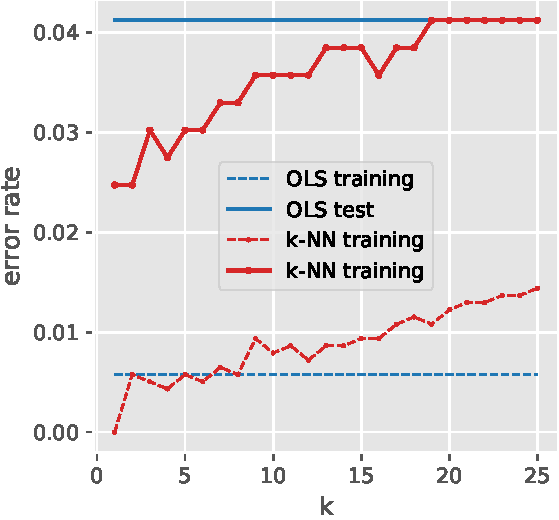
\includegraphics[width=\half]{E2p8_A.pdf}
\end{minipage}\halfspace
\begin{minipage}{\half}
    \centering
    \begin{tabular}{|c|c|c|}
        \hline
        \textbf{Model} & \textbf{Training error} & \textbf{Test error}\\
        \hline
        OLS & 0.58 \% & 4.12 \% \\
        \hline
        1-NN & 0 & 2.47 \% \\
        \hline
        3-NN & 0.50 \% & 3.02 \% \\
        \hline
        5-NN & 0.58 \% & 3.02 \% \\
        \hline
        7-NN & 0.65 \% & 3.30 \% \\
        \hline
        15-NN & 0.94 \% & 3.85 \% \\
        \hline
    \end{tabular}
\end{minipage}